\subsection*{a.4 -- COMSOL validation of the new design}

The new geometry was rebuilt in COMSOL 6.4 with the same modelling recipe
validated in Part~2: 2D plane stress with $t=\SI{200}{\nano\meter}$,
isotropic Si ($E=\SI{170}{\giga\pascal}$, $\nu=0.28$,
$\rho=\SI{2330}{\kilo\gram\per\cubic\meter}$), fixed beam anchors; for the
electromechanical studies the shuttle is a Domain Terminal at \SI{0}{\volt},
the stator floor and fixed-finger walls carry $\Vd$, an Electromechanical
Forces coupling acts on the solids and the air cavity deforms with a
hyperelastic moving mesh. Figure~\ref{fig:p3mesh} shows the mesh.

\begin{figure}[H]
\centering
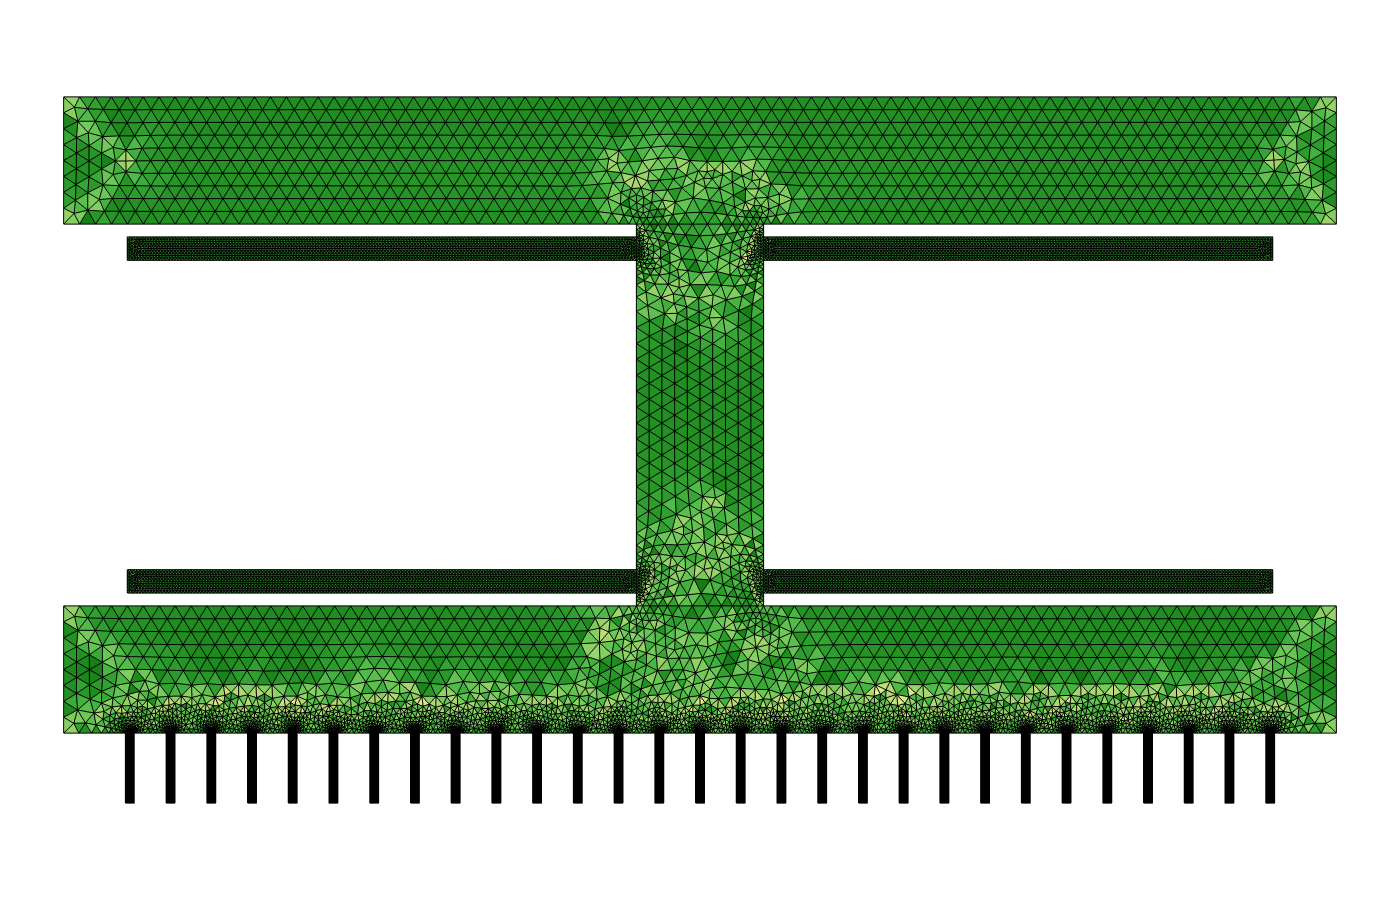
\includegraphics[width=0.8\textwidth]{figures/p3a_model_mesh.png}
\caption{Mesh of the mechanical model (normal refinement, 12\,731 elements).
The element size is refined in the comb region where features are
0.7--\SI{0.9}{\micro\meter}.}
\label{fig:p3mesh}
\end{figure}

\paragraph{(i) Equivalent spring constant.}
A \SI{1}{\micro\newton} test force on the spine along $-y$ gives $k=F/|u_{y}|$
(Table~\ref{tab:p3kconv}). The FEM value, $k=\SI{12.50}{\newton\per\meter}$,
is 7.1\% below the analytical $4EtW_{b}^{3}/L_{b}^{3}=\SI{13.45}{\newton\per\meter}$
-- the same plate-compliance and shear effects quantified in Part~2 (there
$-8.7\%$). The deviation is smaller here because the slimmer plates
contribute less of the total compliance budget relative to the much softer
beams. The design anticipated this with the Part-2-calibrated factor 0.92
($\to\SI{12.38}{\newton\per\meter}$, within 1\% of the FEM).

\begin{table}[H]
\centering
\small
\caption{Mesh convergence of the spring constant.}
\label{tab:p3kconv}
\begin{tabular}{lcc}
\toprule
mesh & elements & $k$ (\si{\newton\per\meter})\\
\midrule
coarse & 4\,429  & 12.578\\
normal & 12\,731 & 12.525\\
fine   & 40\,916 & 12.501\\
\bottomrule
\end{tabular}
\end{table}

\paragraph{(ii) First five eigenmodes.}
Table~\ref{tab:p3modes} and Fig.~\ref{fig:p3modes} summarize the
eigenfrequency analysis (frequencies converged to 0.1\% between two mesh
refinements). The fundamental mode at \textbf{\SI{521.7}{\kilo\hertz}}
satisfies $f_{r}>\SI{500}{\kilo\hertz}$ \checkmark. The analytical prediction
(539 kHz) is 3.2\% high -- exactly the softer FEM spring,
$\sqrt{12.50/13.45}=0.964$; the FEM modal mass $k/\omega_{1}^{2}=\SI{1.163}{\pico\gram}$
matches the lumped estimate (\SI{1.175}{\pico\gram}) to 1\%. Unlike Part~2,
where the comb fingers formed a band at \SI{3.3}{\mega\hertz}, the redesigned
stubby fingers have internal modes near \SI{32}{\mega\hertz} and disappear
from the low spectrum entirely; modes 2--5 are plate rotation/bending modes,
the family the side-stability constraints deliberately keep stiff. The
separation $f_{2}/f_{1}=5.1$ means the device behaves as a clean single-mode
actuator over a wide band.

\begin{table}[H]
\centering
\small
\caption{First five eigenfrequencies (fine mesh).}
\label{tab:p3modes}
\begin{tabular}{clc}
\toprule
mode & character & $f$ (\si{\kilo\hertz})\\
\midrule
1 & shuttle translation along $y$ (actuation mode)        & 521.7\\
2 & spine in-plane rotation, fingers swinging laterally   & 2\,634.8\\
3 & bar in-plane rotation (symmetric partner of mode 2)   & 2\,786.1\\
4 & symmetric in-plane bending of the plate tips          & 5\,519.3\\
5 & higher-order plate bending with beam second modes     & 7\,616.5\\
\bottomrule
\end{tabular}
\end{table}

\begin{figure}[H]
\centering
\begin{subfigure}{0.49\textwidth}
  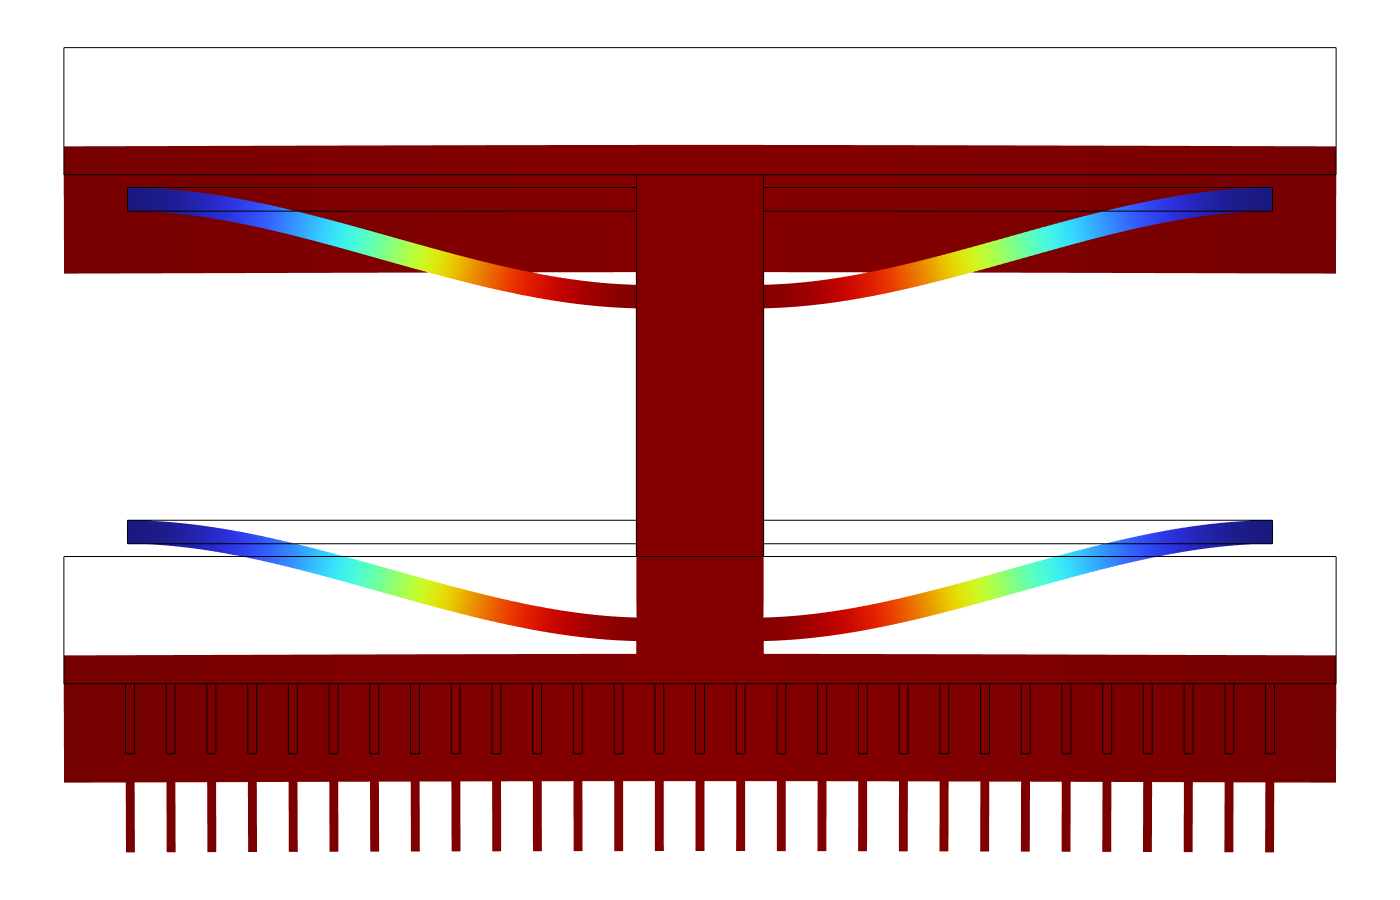
\includegraphics[width=\textwidth]{figures/p3a_mode1_522kHz.png}
  \caption{mode 1: \SI{521.7}{\kilo\hertz}}
\end{subfigure}
\begin{subfigure}{0.49\textwidth}
  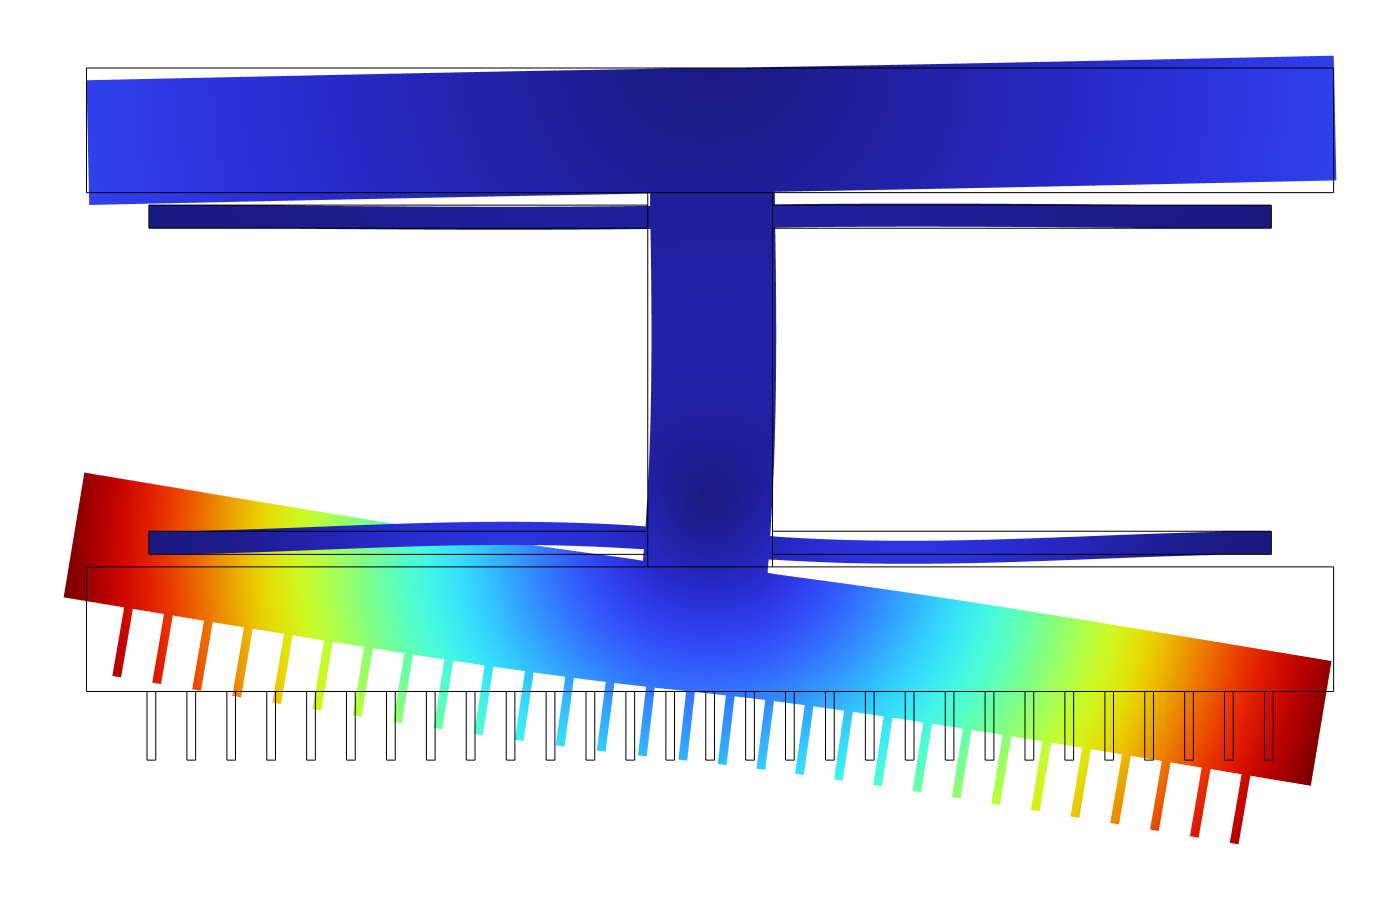
\includegraphics[width=\textwidth]{figures/p3a_mode2_2635kHz.png}
  \caption{mode 2: \SI{2634.8}{\kilo\hertz}}
\end{subfigure}\\[2pt]
\begin{subfigure}{0.49\textwidth}
  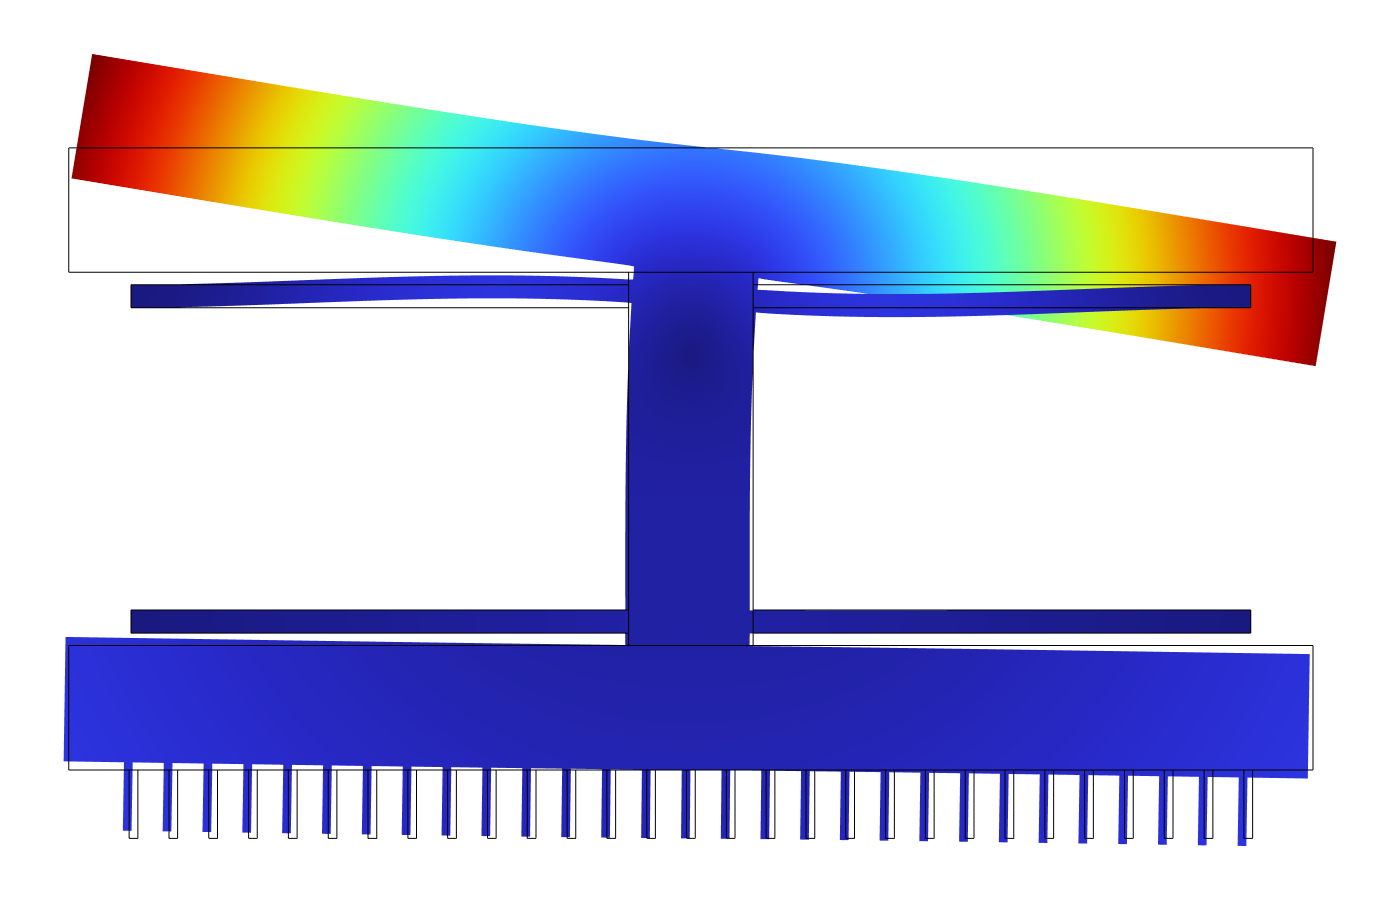
\includegraphics[width=\textwidth]{figures/p3a_mode3_2786kHz.png}
  \caption{mode 3: \SI{2786.1}{\kilo\hertz}}
\end{subfigure}
\begin{subfigure}{0.49\textwidth}
  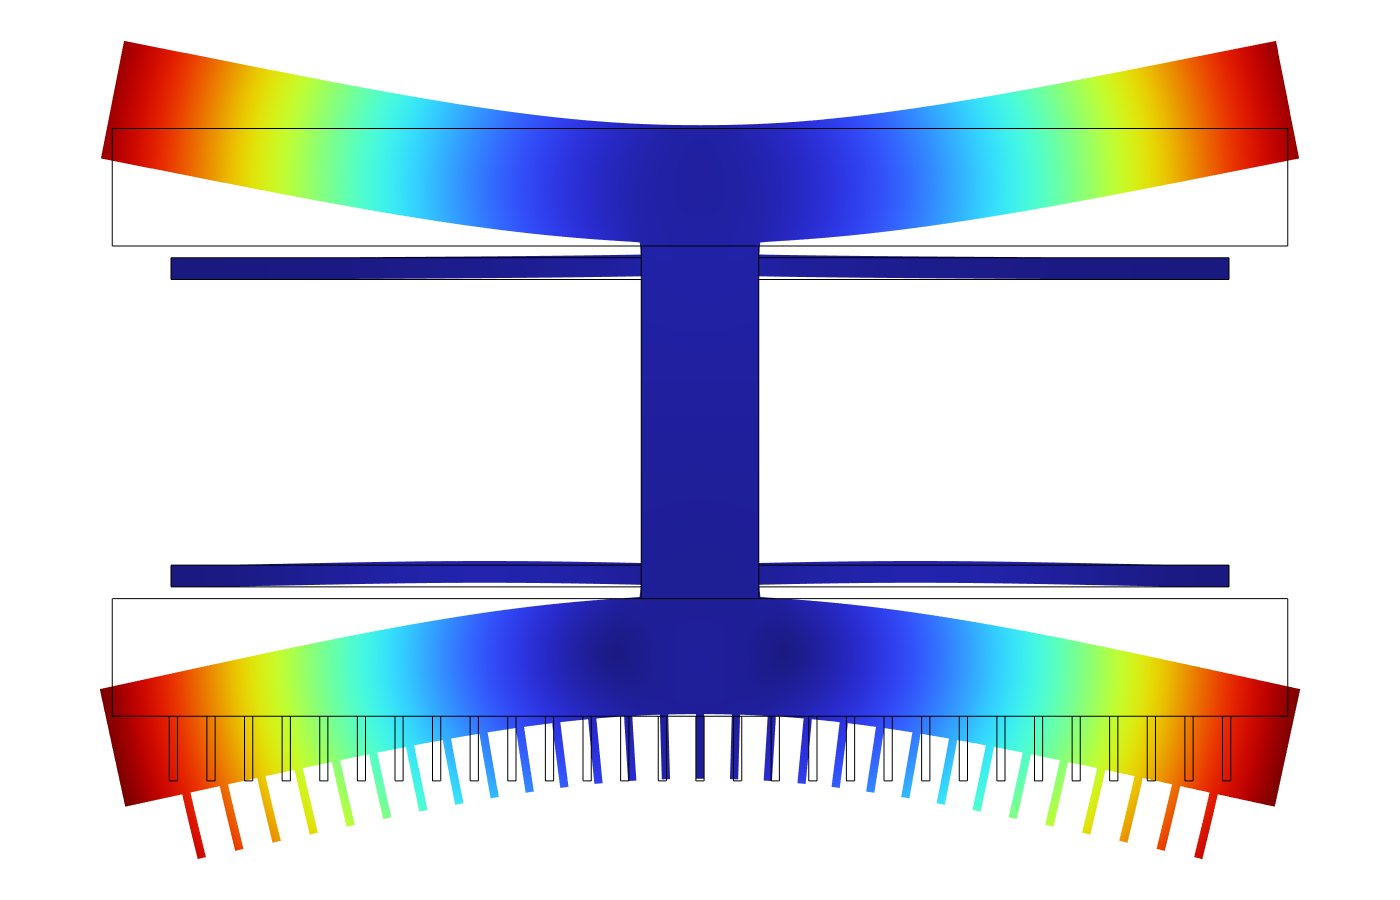
\includegraphics[width=\textwidth]{figures/p3a_mode4_5519kHz.png}
  \caption{mode 4: \SI{5519.3}{\kilo\hertz}}
\end{subfigure}\\[2pt]
\begin{subfigure}{0.6\textwidth}
  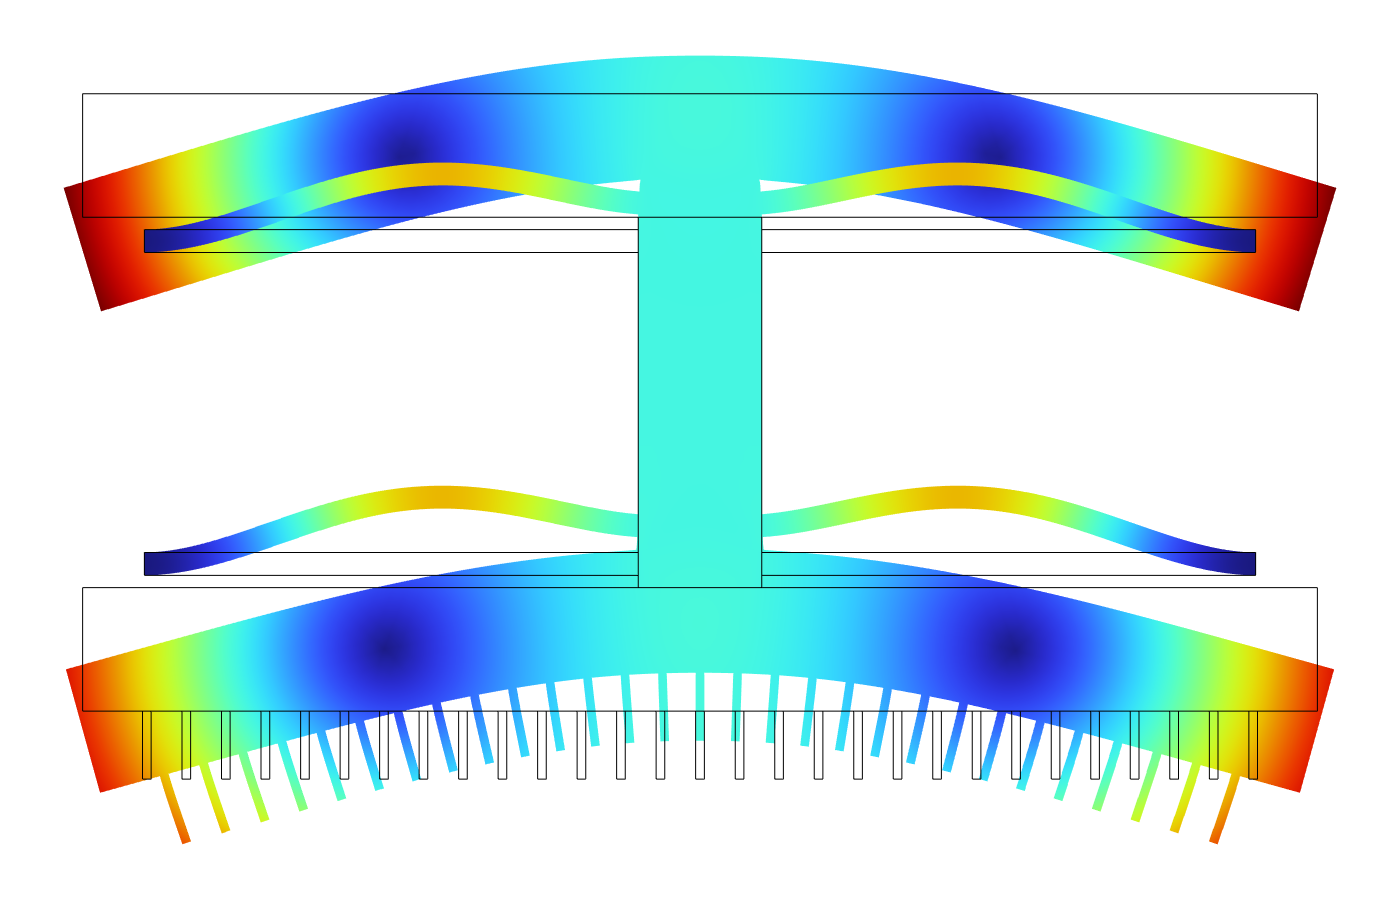
\includegraphics[width=\textwidth]{figures/p3a_mode5_7616kHz.png}
  \caption{mode 5: \SI{7616.5}{\kilo\hertz}}
\end{subfigure}
\caption{2D modal displacement maps of the first five modes of the optimized
design.}
\label{fig:p3modes}
\end{figure}

\paragraph{(iii) Maximum DC displacement at the intended operating voltage.}
A stationary continuation sweep $\Vd=0\to\SI{760}{\volt}$ (steps of
\SI{10}{\volt}, \SI{627}{\volt} included) tracks the stable branch
(Fig.~\ref{fig:p3vsweep}, left). At the design operating voltage,
\begin{equation*}
  x(\SI{627}{\volt})_{\mathrm{FEM}}=\SI{0.919}{\micro\meter}
  \quad\text{toward the comb (away from the waveguide)},
\end{equation*}
vs the analytical optimum $1/(2b)=\SI{1.667}{\micro\meter}$ -- 45\% below the
lumped prediction. The sweep data identify two physical causes that the
ideal-comb model misses:
\begin{enumerate}
\item \emph{Shallow-engagement (fringe-regime) comb constant.} The
      force-implied $(dC/dx)_{\mathrm{eff}}=2k_{\mathrm{FEM}}|u_{y}|/V^{2}$
      is only $\approx\SI{71}{\pico\farad\per\meter}$ at low bias, vs the
      ideal $N\varepsilon_{0}t/h=\SI{114}{\pico\farad\per\meter}$
      (Fig.~\ref{fig:p3vsweep}, right). With $d_{0}=\SI{1}{\micro\meter}$
      the rest overlap is only $1.1h$: the parallel-plate flank field is not
      yet developed, and the constant-$dC/dx$ assumption only becomes valid
      at engagements of a few $h$. (Part 2 never exposed this -- its
      $d_{0}=\SI{19}{\micro\meter}$ comb was deeply engaged.)
\item \emph{Beam stress stiffening.} At micron stroke the fixed--guided
      beams stretch ($x/W_{b}\approx0.5$--$0.9$); the prestressed
      eigenfrequencies (Fig.~\ref{fig:p3soft}) show $f_{1}$ \emph{rising}
      from \SI{522}{\kilo\hertz} at \SI{0}{\volt} to \SI{586}{\kilo\hertz}
      at \SI{450}{\volt} -- a $+26\%$ tangent-stiffness increase that
      further suppresses $dx/dV$.
\end{enumerate}

\begin{figure}[H]
\centering

\includegraphics[width=\textwidth]{figures/p3a_q4iii_vsweep.pdf}
\caption{Left: displacement vs bias -- FEM continuation sweep against the
analytical curve (with both $k_{\mathrm{ana}}$ and $k_{\mathrm{FEM}}$). The
sweep converges through \SI{760}{\volt} with no fold: no pull-in in the
operating range. Right: the force-implied effective comb constant, showing
the shallow-engagement deficit relative to the ideal $N\varepsilon_{0}t/h$.}
\label{fig:p3vsweep}
\end{figure}

The consequence is a shift, not a loss: the FEM-derived low-frequency
sensitivity $|H|(V)=S_{\phi}(g_{0}+x)\,dx/dV$ (Fig.~\ref{fig:p3sensfem})
reaches \SI{35.7}{\milli\radian\per\volt} at the design's \SI{627}{\volt}
and \SI{54.9}{\milli\radian\per\volt} at \SI{760}{\volt}, still rising --
the optimum displacement $1/(2b)$ is reached near \SI{870}{\volt} by
extrapolation. Because $S(x)\propto\sqrt{x}\,e^{-bx}$ is very flat around
its maximum, operating anywhere on the 750--900 V plateau recovers the
designed sensitivity to within a few percent, and the redesign goal -- a
reachable sensitivity maximum -- is preserved, since pull-in moves up even
faster (see the pull-in verification below).

\begin{figure}[H]
\centering

\includegraphics[width=0.8\textwidth]{figures/p3a_sensitivity_fem.pdf}
\caption{Low-frequency modulation sensitivity vs bias: analytical
(ideal comb) and FEM-derived from the static sweep,
$S_{\phi}(g_{0}+x)\,dx/dV$. The three FEM regimes are visible: the
fringe-deficit linear rise, the stress-stiffening plateau around
400--600 V, and the recovery at deep engagement. The FEM optimum lies near
\SI{870}{\volt}, beyond the design value but still far below pull-in.}
\label{fig:p3sensfem}
\end{figure}

\paragraph{(iv) Maximum DC acceleration without hitting the waveguide.}
A body load $\rho a$ on all suspended silicon ($+y$, toward the waveguide)
at $\Vd=0$ (worst case -- bias only adds clearance) gives contact,
$u_{y,\mathrm{bar}}=+g_{0}$, at
\begin{equation*}
  a_{\mathrm{max,DC}} = \SI{2.12e6}{\meter\per\second\squared}
  = 2.16\times10^{5}\,g
\end{equation*}
(verification solve at $a_{\mathrm{max}}$: residual $-0.6\%$, the small
deficit being the onset of geometric stiffening). The lumped check
$k_{\mathrm{FEM}}g_{0}/m_{\mathrm{static}}=\SI{2.10e6}{\meter\per\second\squared}$
agrees to 1.3\%; the fully analytical value
($k_{\mathrm{ana}}$) is 6\% high, again the spring softening. Note that this
quasi-static number is not the binding requirement: the design constraint was
the worst-case-frequency AC value
$a_{0,\mathrm{max}}(\omega_{r})=g_{0}\omega_{r}^{2}/Q
=\SI{2.8e4}{\meter\per\second\squared}>\SI{2e4}{\meter\per\second\squared}$
\checkmark, which is $Q\approx81$ times smaller than the DC limit because
resonance amplifies the base excitation.

\paragraph{(v) Step response and rise time.}
Rayleigh damping is set to stiffness-proportional,
$\beta_{dK}=1/(2\pi f_{1}Q)$ with the analytical $Q=80.7$ at the FEM
$f_{1}=\SI{521.7}{\kilo\hertz}$, and a \SI{1}{\micro\newton} force step is
applied to the spine from rest (Fig.~\ref{fig:p3step}). The final
displacement, \SI{79.7}{\nano\meter}, matches the static $F/k_{\mathrm{FEM}}$
to 0.4\%. The 10--90\% \textbf{rise time is \SI{0.30}{\micro\second}} -- the
force step accelerates the \SI{1.18}{\pico\gram} shuttle within a fraction of
the \SI{1.92}{\micro\second} oscillation period, in agreement with the
undamped $1-\cos\omega_{1}t$ first-rise estimate
$1.02/\omega_{1}=\SI{0.31}{\micro\second}$. Because the device is strongly
underdamped ($\zeta=1/2Q=6.2\times10^{-3}$), the response then rings at
$f_{1}$ and \textbf{settles to 5\% in \SI{148.6}{\micro\second}}, in
agreement with the analytical envelope estimate
$t_{s}=\ln(20)/(\zeta\omega_{1})=\SI{147.5}{\micro\second}$ (0.7\%).
Compared with Part 2 (\SI{158}{\micro\second} at $f_{1}=\SI{496}{\kilo\hertz}$,
$Q=83$): $t_{s}\propto Q/f_{1}$, so the slightly faster, slightly less
damped new device settles marginally sooner. For the modulator application
the rise time is the relevant number; the long ring-down only matters as a
recovery time after shocks or bias steps.

\begin{figure}[H]
\centering

\includegraphics[width=\textwidth]{figures/p3a_q4v_step_response.pdf}
\caption{Force-step response of the optimized device
(\SI{1}{\micro\newton} on the spine, $Q=80.7$). Left: full window with the
$\pm5\%$ band and settling time. Right: the first ten microseconds with the
10--90\% rise markers.}
\label{fig:p3step}
\end{figure}

\paragraph{Pull-in verification.}
Because the whole design hinges on $\VDCMAX<\VPI$, two checks beyond the
assignment list were run. First, the static continuation sweep converges
through \SI{760}{\volt} with no fold -- no pull-in anywhere in or near the
operating range. Second, prestressed eigenfrequencies vs bias (a
continuation-ramped stationary solve followed by an eigenfrequency study at
each bias) expose which mode loses stiffness (Fig.~\ref{fig:p3soft}):

\begin{table}[H]
\centering
\small
\caption{Prestressed eigenfrequencies vs DC bias.}
\label{tab:p3soft}
\begin{tabular}{ccc}
\toprule
$\Vd$ & $f_{1}$ (actuation) & $f_{2}$ (spine rotation = side mode)\\
\midrule
\SI{0}{\volt}   & \SI{522.2}{\kilo\hertz} & \SI{2636.7}{\kilo\hertz}\\
\SI{400}{\volt} & 557.4 ($+6.7\%$)        & 2\,512.7 ($-4.7\%$)\\
\SI{627}{\volt} & \textbf{675.2 ($+29\%$)} & 2\,170.5 ($-18\%$)\\
\SI{760}{\volt} & 584.5                   & 1\,519.5 ($-42\%$)\\
\bottomrule
\end{tabular}
\end{table}

$f_{1}$ is non-monotonic: stress stiffening dominates up to
$\approx\SI{650}{\volt}$ ($+29\%$), then electrostatic softening takes over;
$f_{1}^{2}\to0$ extrapolates to $\approx\SI{1100}{\volt}$. The critical
channel is mode 2 -- the spine-rotation (side) mode -- whose
$f_{2}^{2}\to0$ extrapolation gives $\VPI^{\mathrm{FEM}}\approx\SI{876}{\volt}$.
Three conclusions: (i) the analytically designed side pull-in
(\SI{723}{\volt}) is 17\% conservative, as expected from the Dunkerley
combination; (ii) the \emph{character} of the instability -- lateral, through
the comb's negative lateral stiffness, not the axial tip fold -- confirms the
Part-2 lesson and the constraint set used in the optimization; and (iii) the
ordering is as designed,
$V_{\mathrm{op}}\;(627) < \VPI^{\mathrm{side}}\;(\approx876) <
\VPI^{\mathrm{axial}}\;(\approx1100\,\mathrm{V})$, so \textbf{all four
assignment constraints hold in the FEM}: $f_{r}=\SI{521.7}{\kilo\hertz}$,
$\VPI\approx\SI{876}{\volt}>\SI{200}{\volt}$, $\VDCMAX<\VPI$ (28\% margin),
and $a_{0,\mathrm{max}}(\omega_{r})=\SI{2.8e4}{\meter\per\second\squared}$.

\begin{figure}[H]
\centering

\includegraphics[width=0.8\textwidth]{figures/p3a_eig_softening.pdf}
\caption{Prestressed eigenfrequencies vs bias. Mode 2 (spine rotation, the
side channel guarded by the design constraints) softens toward pull-in at
$\approx\SI{876}{\volt}$; mode 1 first \emph{stiffens} ($+29\%$ at the
operating point, beam stress stiffening) before electrostatic softening
takes over.}
\label{fig:p3soft}
\end{figure}

\paragraph{Summary of deviations and possible second iteration.}
Table~\ref{tab:p3dev} condenses the analytic$\,\leftrightarrow\,$FEM
comparison. The two systematic effects -- shallow-engagement comb force and
beam stress stiffening -- \emph{shift} the sensitivity optimum from 627 V
into the 750--900 V range without destabilizing it, because the same
stiffening physics raises pull-in even faster. A second design iteration
could recover the lower-voltage optimum by deepening the rest overlap
($d_{0}\to2.5$--\SI{3}{\micro\meter}, restoring the ideal $dC/dx$) and
lengthening the beams at constant $k$ (reducing $x/W_{b}$ and the
hardening), at a modest cost in side-stability margin; since all assignment
constraints are already met, this is left as a documented refinement.

\begin{table}[H]
\centering
\small
\caption{Analytical model vs COMSOL: the a.4 comparison at a glance.}
\label{tab:p3dev}
\begin{tabularx}{\textwidth}{lllX}
\toprule
quantity & analytic & FEM & cause of deviation\\
\midrule
$k$ & \SI{13.45}{\newton\per\meter} & \SI{12.50}{\newton\per\meter} ($-7\%$) & plate compliance, shear\\
$f_{r}$ & \SI{538.6}{\kilo\hertz} & \SI{521.7}{\kilo\hertz} ($-3\%$) & softer $k$\\
$x(\SI{627}{\volt})$ & \SI{1.667}{\micro\meter} & \SI{0.919}{\micro\meter} ($-45\%$) & fringe-regime $dC/dx$ ($\times0.62$) + stress stiffening ($+26\%$ $k_{\mathrm{tan}}$)\\
peak $|H|$ & \SI{73.9}{\milli\radian\per\volt} @ 627 V & $\approx\SI{55}{\milli\radian\per\volt}$ @ 760 V, rising & same two causes; flat $S(x)$ limits the loss\\
$\VPI$ (side) & \SI{723}{\volt} & $\approx\SI{876}{\volt}$ ($+17\%$) & Dunkerley conservatism; stiffening aids stability\\
$a_{\mathrm{max,DC}}$ & \SI{2.26e6}{\meter\per\second\squared} & \SI{2.12e6}{\meter\per\second\squared} ($-6\%$) & softer $k$\\
$t_{s}$, rise & \SI{147.5}{\micro\second}, \SI{0.31}{\micro\second} & \SI{148.6}{\micro\second}, \SI{0.30}{\micro\second} & agreement $\le1\%$\\
\bottomrule
\end{tabularx}
\end{table}
